\section*{Problema 4}

\textbf{Este ejercicio es sobre el uso de métodos de clasificación para detectar billetes falsos:}

\begin{figure}[H|]
	\centering
	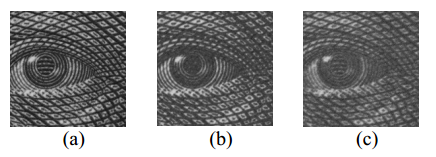
\includegraphics[width=16cm]{Graphics/Problema_04/image01.png}
	\caption{(a) (parde de) un billete de verdad, (b) billete falso de alta calidad, (c) billete falso de baja calidad.}
\end{figure}


\textbf{En el paper que se anexa a la tarea se resume cada billete con cuatro caracteristicas (varianza, skewness, curtosis y entropía) extraidas de la forma del histograma de los coeficientes de la transformación de Wavelet. Los histogramas a continuación muestran como cambia la forma cuando el billete ya no es auténtico.}

\begin{figure}[H|]
	\centering
	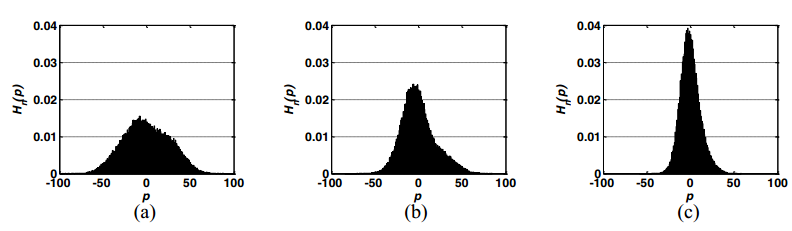
\includegraphics[width=16cm]{Graphics/Problema_04/image02.png}
	\caption{(a) histograma de los coeficientes de un billete de verdad, (b) billete falso de alta calidad, (c) billete falso de baja calidad.}
\end{figure}

\textbf{Se anexo el conjunto de datos. La última columna indica si el billete es falso o no.}

\begin{itemize}
	\item Resume, visualiza y analiza los datos
	\item Construye algunos clasificadores interesantes basados en SVM (explora diferentes kerneles). Estima su poder predictivo, para eso divide muchas veces los datos en conjunto de prueba y de entrenamiento y cuenta falsos positivos y falsos negativos. Las instrucciones básicas de SVM para R y Python están al fianl de \file{recpat4b.pdf}
\end{itemize}
